% \documentclass[dvipdfmx, a4paper, 11pt]{jsarticle}%A4用紙縦,明朝(デフォルト)11ポイント
\documentclass[dvipdfmx,titlepage, 11pt, a4paper]{jsarticle}%A4用紙縦,明朝(デフォルト)11ポイント
\usepackage[top=30truemm,bottom=20truemm,left=20truemm,right=20truemm]{geometry}%余白調整
\usepackage{template}

%%%====================================================================================================================================
\renewcommand{\thesection}{問題番号\ \fbox{\ \ \arabic{section}\ \ }}
\renewcommand{\thesubsection}{科目名}
\renewcommand{\thesubsubsection}{\thesection}
\titleformat*{\section}{\LARGE\mcfamily}%章のタイトルの文字の大きさを通常サイズに設定(明朝体で)
\titlespacing*{\section}{0pt}{*0}{0pt}%章番号の後の空白行の削除
\titleformat*{\subsection}{\Large\mcfamily}%節のタイトルの文字の大きさを通常サイズに設定(明朝体で)
\titlespacing*{\subsection}{0pt}{*0}{0pt}%節番号の後の空白行の削除
\titleformat*{\subsubsection}{\large\mcfamily}%小節のタイトルの文字の大きさを通常サイズに設定(明朝体で)
\titlespacing*{\subsubsection}{0pt}{*0}{0pt}%小節番号の後の空白行の削除

\makeatletter
%章番号付きコード番号
\AtBeginDocument{
  \renewcommand*{\thelstlisting}{\arabic{section}.\arabic{lstlisting}}%
  \@addtoreset{lstlisting}{section}
}

%章番号付き表番号
\renewcommand{\thetable}{%
    \arabic{section}.\arabic{table}%
}
\@addtoreset{table}{section}%

%章番号付き図番号
\renewcommand{\thefigure}{%
	\arabic{section}.\arabic{figure}%
      }%
\@addtoreset{figure}{section}%

%章番号付き式番号
\renewcommand{\theequation}{%
	\arabic{section}.\arabic{equation}%
}%
\@addtoreset{equation}{section}%

\renewcommand{\p@enumiii}{}% 箇条書きの参照時の番号の変更(2(親の番号)a(子の番号)→aだけに)
\renewcommand{\p@enumii}{}% 箇条書きの参照時の番号の変更(2a→aだけに)
\makeatother
%%%====================================================================================================================================

%%%====================================================================================================================================
%%ページのレイアウト設定
%\pagestyle{fancy}
\renewcommand{\sectionmark}[1]{\markboth{}{\thesection\ #1}}%                   %\rightmarkにセクション名を格納
\renewcommand{\subsectionmark}[1]{\markboth{#1}{\rightmark}}%   %\leftmarkにサブセクション名を格納
%[]は省略可で省略すると{}で指定された内容が偶数ページ奇数のどちらにも適用される.
% \renewcommand{\headrulewidth}{0pt} %ヘッダの罫線を消す 
%\fancyfoot{}%                        %clear all footer fields
\lhead{\leftmark}%                   %左側ヘッダの定義[<偶数ページ>]{<奇数ページ>}
\chead{\large \bf 2019年9月・2020年4月入学試験問題\\大学院基幹理工学研究科修士課程情報理工・情報通信専攻}%                            %中央ヘッダの定義[<偶数ページ>]{<奇数ページ>}
\rhead{\rightmark}%                  %右側ヘッダの定義[<偶数ページ>]{<奇数ページ>}
\lfoot{早稲田2019年度解答例}%       %左側フッターの定義[<偶数ページ>]{<奇数ページ>}
\cfoot{\thepage}%                    %中央フッターの定義[<偶数ページ>]{<奇数ページ>}
\rfoot{文殊の知恵}%                  %右側フッターの定義[<偶数ページ>]{<奇数ページ>}
\renewcommand{\headrulewidth}{0.1pt}%%ヘッダの線の太さ 
\renewcommand{\footrulewidth}{0.1pt}%%フッターの線の太さ
%%%====================================================================================================================================

\makeindex%索引用

\renewcommand{\refname}{}%参考文献の文字を非表示にする
\title{\Huge 早稲田2019年度解答例\\[10mm]}
\author{{\LARGE 文殊の知恵}\\[1mm]\LARGE 中田昌輝}
\date{}

\begin{document}
\maketitle
%\tableofcontents % 目次
\pagenumbering{roman}%目次のページ番号のスタイルをローマ数字にする
\newpage
\setcounter{tocdepth}{3}%章節の深さを3にするsubsubsectionまで
\pagenumbering{arabic}%他のページ番号は通常の数字にする.
\section{}
\subsection{情報基礎}
\subsubsection{問題文}
以下の問(1)〜(3)に答えよ.
\begin{enumerate}[(1)]
  \setlength{\itemsep}{10pt}  
\item 集合$\Sigma=\{0,1\}$について, $\Sigma$上の記号列全体の集合(the set of all strings over $\Sigma$)を$\Sigma^{\ast}$で表す。
  \begin{enumerate}[(${1}-$a)]
    \setlength{\itemsep}{15pt}   
  \item 次の文が正しい定義となるように空欄【\ \ \ 】を埋めよ。
    \begin{center}
      $\Sigma$上の言語(language over $\Sigma$)とは$\Sigma^{\ast}$の【\hspace{20pt} 】のことである。
    \end{center}
  \item $\Sigma$上の言語$A,B$が等しいとはどういうことか書け。
  \item 言語$\{0^{2n}1|n\geq 1\}$を表現する正則表現(regular expression)を書け。
  \item 次の文が「言語$L=\{0^{n}1^{n}|n\geq 1\}$は正則言語ではない」ことの証明となるように, 空欄【\ \ \ 】を埋めよ。\\[0.5cm]
    \begin{minipage}{13cm}
      $L$を認識(recognize)する決定性有限オートマトン(deterministic finite automaton)の状態(state)の数を$m$とすると,【\hspace{20pt}】が受理(accept)される過程でこのオートマトンが入る最初の$m+1$個の状態$q_{0},q_{1},q_{2},...,q_{m}$のうち2つは同じ状態だから, それらを$q_{i},q_{j}(0\leq i<j\leq m)$とすると, $0^{m-(j-i)}1^{m}\in L$となり矛盾する。
    \end{minipage}
  \end{enumerate}
  \hspace{1cm}
  
\item 記号表(symbol table)とは, キー(key)を持つ項目(item)からなるデータ構造(data structure)であり, 次の2つの基本操作(basic operations)を持つ。
  \begin{itemize}
  \item[] 新しい項目を挿入(insert)する
  \item[] 与えられたキーを持つ項目を探索(search)する
  \end{itemize}
  次の表は, 記号表における挿入コストと探索コストを表したものである。ここで, 記号表中の項目の個数を$N$とし, コストとは$N$の関数としておおよその計算時間を表している. 空欄(a)〜(e)に\underline{もっとも}ふさわしいものを, 下の選択肢(ア)〜(オ)から選べ。同じ選択肢を複数回選んでもよい。\\
  \begin{center}
    \begin{tabular}{|l|cc|ccc|} \hline
      \multirow{3}{*}{実装方法}&\multicolumn{2}{|c|}{最悪の場合}&\multicolumn{3}{|c|}{平均の場合} \\ \cline{2-6}
                               &\multirow{2}{*}{挿入}&\multirow{2}{*}{挿入}&\multirow{2}{*}{挿入}&成功&不成功\\ 
                               &&&&探索&探索 \\ \hline
      逐次探索&$N$&(a)&$N/2$&$N/2$&(b)\\
      2分探索木&(c)&$N$&$\log_{2}N$&(d)&(e)\\ \hline
    \end{tabular}
  \end{center}
  \vspace{0.5cm}
  
  \noindent 選択肢:\ (ア)1\hspace{10pt} (イ)$N$\hspace{10pt} (ウ)$N/2$\hspace{10pt} (エ)$\log_{2}N$\hspace{10pt} (オ)$N\log_{2}N$
  
  %\newpage
  \begin{minipage}[t]{8cm}
  \item 右図のプログラム片(code fragment)を考える。関数(fuction)sort1(L,R), sort2(L,R), sort3(L,R)はいずれも, グローバルスコープの配列Aに格納されている値A$[$L$]$,...,A$[$R$]$を昇順(ascending order)に整列(sort)をすることをめざしている。ただし引数L,RがL$<$Rを満たし, A$[$L$]$,...,A$[$R$]$がAの定義範囲内となるように呼ばれるものとする。以下, これら3関数の整列と呼ぶ.
    \begin{enumerate}[({3}$-$a)]
    \item 各整列関数の目的を熟考して, 正しく完成させるため, 右図中の空欄【あ】, 【い】, 【う】を適切に埋めよ。
    \item 3つの整列関数が正しく完成したとき, 最も早いものの漸近時間計算量(asymptotic time complexity)は何か。整列する要素数を$n$とせよ.
    \item 3つの整列関数が正しく完成したとき, そのうち1つは, すでにほとんど昇順に整列している入力列について他の2つより速い。その関数はどれか。
    \item 3つの整列関数のうち, 正しく完成したとき安定(stable)であるものをすべて答えよ。
    \item 右図の3つの整列関数のうち1つは誤りを含み, A$[$L$]$,...,$[$R$]$の範囲外の配列を参照してしまう。
      
      \begin{enumerate}[i)]    
      \item 誤りのある箇所の行番号(line number)を答えよ。
      \item 誤りを含む整列関数を実行した場合, 最初に範囲外の配列要素を参照する箇所の行番号を答えよ。
      \end{enumerate}
      
    \end{enumerate}
  \end{minipage}
  \hfill
  \begin{minipage}[t]{8.5cm}
    \begin{lstlisting}
 1 fun exch(i,j)
 2     t←A[i]
 3     A[i]←A[j]
 4     A[j]←t
 5 end fun
 6
 7 fun compexch(i,j)
 8     if (A[j] < A[i])
 9         exch(i,j)
10     end if
11 end fun
12
13 fun sort1(L, R)
14     i←L
15     while (i < R)
16         min←i
17         j← i + 1
18         while(j ≦R)
19             if (A[j] < 【あ】)
20                 min←j
21             end if
22             j←j + 1
23         end while
24         exch(i, min)
25         i←i+1
26     end while
27 end fun
28
29 fun sort2(L, R)
30     i←L
31     while (i < R)
32         j←R
33         while(j > i)
34             compexch(j-1,【い】)
35             j←j-1
36         end while
37         i←i+1
38     end while
39 end fun
40
41 fun sort3(L, R)
42     i←R
43     while(i≧L)
44         compexch(i-1, i)
45         i←i-1
46     end while
47     i←L+2
48     while(i≦R)
49         j←【う】
50         v←A[i]
51         while(v < A[j-1])
52             A[j]←A[j-1]
53             j←j-1
54         end while
55         A[j]←v
56         i←i+1
57     end while
58 end fun
    \end{lstlisting}
  \end{minipage}
\end{enumerate}
\newpage

\subsubsection{解答例}
\begin{enumerate}[(1)]
  \setlength{\itemsep}{15pt}   
\item 情報数学の分野である.
  \begin{enumerate}[({1}$-$a)]
    \setlength{\itemsep}{15pt}   
  \item $\Sigma$上の言語とは$\Sigma^{\ast}$からある特定の条件を満足する記号列だけを集めた集合であるので空欄に入れるべき語句は\underline{\bf 部分集合}である.
  \item $\Sigma$上の言語$A,B$が等しいとは同じ記号列の集合であるということであるので, \\\underline{\bf 言語$A$のみを受理するオートマトンと言語$B$のみを受理するオートマトンが等価であるということである}.
  \item 0が偶数回並んだあと, 1が来る文字列を正則表現に変えればいいので, \underline{\bf $(00)^{\ast}1$}
  \item この言語$L$のみを受理するオートマトンが存在しないということである. これはオートマトンが何文字同じ文字を読み込んだかをカウントする機能がないためである(特定の文字数をカウントすることは可能である). したがって$n$回0を読み込んだと記憶を保持することができないので, 1を$n$回読み込むようにすることは不可能である. これを証明すると同じ状態が複数回出てしまうことを用いて背理法で示す. よって, 空欄に入れるべき語句は\underline{\bf $0^{m}1^{m}$}である.
  \end{enumerate}
\item アルゴリズムとデータ構造の分野である.
  \begin{enumerate}[(a)]
  \item 逐次探索は順番に配列を参照していくが探索において最悪の場合は目的のものが最後に存在する場合であるので$N$, つまり\underline{\bf (イ)}.
  \item 整列した配列を使うので, 目的の値が飛ばされていたら不成功であると判断できるので成功探索と同様に$N/2$, つまり\underline{\bf (ウ)}.
  \item 2分探索木で最悪の場合は挿入された順番が整列された値であった場合である. これは2分木にならず右肩下がりまたは右肩上がりのどちらかの木になってしまう. このあと挿入されるとき一番根から離れた場所に挿入する(一番子どもの節点)場合は特に最悪で, すべての要素を見ることとなるので$N$, つまり\underline{\bf (イ)}.
  \item 平均の場合は平衡状態が取れている二分木探索と捉えることができる. このとき成功探索は高さが$\log_{2}N$となるので$\log_{2}N$, つまり\underline{\bf (エ)}.
  \item 不成功探索も成功探索と同様に考えることができるので, $\log_{2}N$, つまり\underline{\bf (エ)}.
  \end{enumerate}
\item exch関数について, これはよく見るswap関数である. つまり配列の添字を付け替える, 値を入れ替える関数である. つぎにcompexchは値の大小が逆であった場合はexch関数を呼び出して値の整列を行っている.
  \begin{enumerate}[({3}$-$a)]
  \item sort1関数についてみてみる. 配列の添字を参照するための変数iを左端つまり一番小さいと思われる配列の添字に代入している. これを左から右まで順に動かすwhile文がみえる. 一旦iを別のところ(min)に格納し, jにiの次の添字を格納している. その次にjが右端になるまで比較を行っている. ここで最小値を見つけ次第jの値をminにいれて最小値を探していると判断することができる. この最小値が入っている添字は本来, iのところにあるべきであることを考慮すれば【あ】に入るべき語句は\underline{A$[$min$]$}であるとわかる. これは選択ソートである.\\
    つぎにsort2関数についてみてみる. iを左端に, つぎにiが右に行くまでjを右端にするwhile文がみえる. j$>$iとつねにiはj以下という条件で2つめのwhile文を回している. while文内でjを1ずつ減らしていることからiを基準とし, jを右から順々にずらしていることがわかる. つまり左端から順にソートされていくことがわかる.  ここでcompexch関数は大小を比較して入れ替えるというものであった. つまりiのほうがj-1より小さいべきでありjのほうがj-1より大きいべきである. ここでどちらがふさわしいかどうかを考える. iとj-1を入れ替えるソート方法であると不安定になってしまうので, 安定にソートする方法としてはjとj-1を入れ替えるソートである.  【い】に入れるべき語句は\underline{j}であるとわかる. これはバブルソートである.\\
    最後にsort3関数についてみてみる. iを右からみていき左端になるまで一つ前のi-1と入れ替えていることがわかる. これからいえることとしては左端の値がソートされた状態になるということである. つぎにiにL+2を入れた式からみるとiが右端に行くまでjの値を変えている. つまりiを左から揃えていくためのソートされた列か未ソートの列かを区別するための基準となる変数であることがわかる. つまりjを右端から揃えていき, 未ソートの列の左端A$[$i$]$をvにいれることで一つずつ揃えていることが分かる. ゆえに【う】に入れるべき語句は\underline{R}であることがわかる. これは挿入ソートである.
  \item どのソートの計算量も\underline{$O(n^{2})$}である. 平均として$n(n-1)/2$の比較を行う. バブルソートの場合はどのような状況においても$n(n-1)/2$の比較を行う.
  \item すでにほとんど昇順に整列している入力列については挿入ソートは$O(n)$の速さでソートすることが可能である. というのも小さい値が見つかった場合は挿入ソートの場合は配列の添字を一つずつずらして値を挿入するという操作が行われるが, 整列されている場合はその操作がなくなるので早く実行することができる. つまり答えは\underline{\bf sort3}である.
  \item 安定であるかどうかについて, 安定であるものは$1,3,2_{A},2_{B},4$というソートに対し, $1,2_{A},2_{B},3,4$というふうにいかなる状況でもソートされるものを指す. 一方で不安定であるものとは$1,2_{B},2_{A},3,4$というふうに同じ2という数字でも入れ替えが起こってしまうことをいう. この不安定な状況が起こるのは隣同士の値を比較するのではなく離れた場所での値を比較するために起こる. ゆえにバブルソートは隣同士の値を比較するため安定である. また挿入ソートも後方から値を確認していくため, 同じ値におけるソートの入れ替えが起きない. 一方で選択ソートは最小値をとりそれを入れ替えるという方法でソートしていくので離れた場所での値を比較することとなる. そのため安定ではない. ゆえに答えは\underline{\bf sort2, sort3}である.
  \item 見るべきポイントとしては加算や減算処理が行われているときのループ文である.
    \begin{enumerate}[i)]
    \item i≧Lというのをみるとそのあとi-1を関数の引数にとっているのでL-1が参照されることとなる. ゆえに\underline{\bf 43}行.
    \item 関数が実行されるときなので\underline{\bf 44}行.
    \end{enumerate}
  \end{enumerate}
\end{enumerate}
\newpage

\section{}
\subsection{計算機システム}
\subsubsection{問題文}
\vspace{0.6cm}

\begin{center}
  \begin{tikzpicture}[>=stealth]
    \draw[xscale=3.5] (0,0) circle[radius=1];
    \draw[xscale=3.5,very thick] (0,0) circle[radius=1.3];
    \filldraw (3,0.15) rectangle (3.45,0.6);
    \draw[very thick] (3.225,0.375)--(6,0.375);
    \draw[->,thick] (7,-1)--(5.2,0.3);
    \draw(7,-1)--(7,-1) node[below] {\bf アーム};
    \draw[->,thick] (2.5,-2.5)--(1.5,-1);
    \draw(2.5,-2.5)--(2.5,-2.5) node[below] {\bf トラック};
    \draw[->,thick] (3.6,1.7)--(3.3,0.7);
    \draw(3.6,1.7)--(3.6,1.7) node[above] {\bf ヘッド};
    \draw(-2,1)--(-1.6,0.6);
    \draw(-2.5,0.9)--(-2.1,0.5);
    \draw[->,thick] (-3,1.7)--(-2.15,0.9);
    \draw(-3,1.7)--(-3,1.7) node[above] {\bf セクタ};
  \end{tikzpicture}
\end{center}

\noindent 磁気ディスク(Magnetic Disk)とは, 上図に示すようなデータ記憶に磁性体を塗布した円盤を回転させておこなう記憶媒体の名称である。磁気ディスク上のデータの読み書きに関する以下の設問に解答せよ。各円盤上のトラック(Track)数を30, 1つのトラック内のセクタ(Sector)数を100, 円盤は1msで1回転し, アーム(Arm)に取りつけられたヘッド(Head)の移動時間に関してはトラック間の移動に2ms必要とするとする。また, 各セクタは64バイトのデータを格納できるとする。
\begin{enumerate}[(1)]
  \setlength{\itemsep}{15pt}
\item 指定されたセクタを読み出す要求があった場合, そのセクタの読み出しに必要な最悪遅延時間を示せ。その際, 最悪遅延時間の結果の導出過程を示すこと。
\item 1つの円盤上の各トラック名をT1-T30と表現する。今, ホスト計算機から, T20, T5, T25, T13, T1, T19の順にデータの読み込み要求があったとする。この場合, FCFS(First Come First Served)スケジューリングを用いてトラックを読み込んだ場合とSCANスケジューリングを用いて読み込んだ場合のそれぞれのトータルの読み込みに必要な時間を示せ。各トラック内のセクタのアクセス時間に関しては最悪の読み込み時間を想定して計算すること。また, 結果の導出過程に関しても記載すること。初期状態として, ヘッドはT1の位置に移動しているとする。
\item バッファキャッシュ(Buffer Cache)は磁気ディスク内の頻繁に利用するデータを実メモリ内に格納するオペレーティングシステムの機能である。今, 128バイトのデータを読み込む場合, すべてのデータがバッファキャッシュ上に格納できている場合と, 全く存在しない場合の最悪の読み込み時間を示せ。結果の導出過程に関しても記載すること。ここでは, バッファキャッシュのブロックサイズは64バイトとし, 実メモリ1メモリの読み込み/書き出し時間を1$\mu$秒とする。また, バッファキャッシュ上にデータが存在しない場合は, 磁気ディスクからデータを読み出してメモリに格納するものとする。
\item 想定するバッファキャッシュは5ブロック分のメモリが割り当てられるものと考える。ここでは, それぞれのブロックをB1-B5として表現する。また, あるトラック上のセクタS1-S30の一部を読み込む場合を考える。今, S1, S2, S3, S4, S1, S2, S5, S6, S7, S1, S2, S3の順にセクタが読み込まれる場合を考える。この場合, バッファキャッシュを管理するポリシーとしてFIFO(First In First Out)を用いた場合と, LRU(Least Recently Used)を用いた場合で, B1-B5が格納するデータが格納されたセクタ番号がどう変化するかを時系列順に図示せよ。
\end{enumerate}
\subsubsection{解答例}
\begin{enumerate}[(1)]
  \setlength{\itemsep}{15pt}
\item 指定されたセクタを読み出す要求があった際, ヘッドが目的のトラックにいない場合はトラック間の移動が2msであるから最悪の場合は29回トラック間の移動が発生するので$2\times 29=58$msかかることとなる. 次に目的のトラックにいる場合でもセクタが目的の場所ではない場合は円盤が回転する必要があるので, 最悪の場合は1回転する必要があるため求める答えは
  \begin{eqnarray*}
    58+1=59{\rm ms}
  \end{eqnarray*}
\item 各トラック内のセクタのアクセス時間は最悪の読み込み時間を想定するのでセクタの移動は毎回1msかかる. FCFSスケジューリングを用いるので, T1からT20への移動は19回移動する. T20からT5は15回移動し, T5からT25は20回, T25からT13は12回, T13からT1は12回,T1からT19は18回の移動となるので合計で$(19+15+20+12+12+18)=96$回移動することとなる. また各トラックで1回転すると考えれば6回転するので求める答えは
  \begin{eqnarray*}
    96\times 2+6\times 1=198{\rm ms}
  \end{eqnarray*}
  となる.
\item すべてのデータがバッファキャッシュ上に格納できている場合はメモリの読み込みだけで済むので, 128$\mu$秒である. 一方で全く存在しない場合の最悪の読み込み時間はヘッドの移動をして読み込みを行いメモリに書き込む作業が2回行われるので, それにかかる時間は
  \begin{eqnarray*}
    2\times(2\times 29+1)=118{\rm ms}
  \end{eqnarray*}
  読み込みは書き出して読み込むので合計で$4\mu$秒かかるとすれば合計で
  \begin{eqnarray*}
    118{\rm m}+4\mu=118.128{\rm ms}
  \end{eqnarray*}
  となる. 
\item それぞれのブロックにはB1からB5を順番に格納するものとする. するとFIFOはきた順に格納するので以下のように変化する.
  \begin{center}
    \begin{tabular}{|c|c|c|c|c|} \hline
      B1&B2&B3&B4&B5\\ \hline\hline
      S1&&&& \\ \hline
      S1&S2&&& \\ \hline
      S1&S2&S3&& \\ \hline
      S1&S2&S3&S4& \\ \hline
      S1&S2&S3&S4&S5 \\ \hline
      S6&S2&S3&S4&S5 \\ \hline
      S6&S7&S3&S4&S5 \\ \hline
      S6&S7&S1&S4&S5 \\ \hline
      S6&S7&S1&S2&S5 \\ \hline
      S6&S7&S1&S2&S3 \\ \hline
    \end{tabular}
  \end{center}
  一方でLRUを用いた格納方式は以下のように格納される.
  \begin{center}
    \begin{tabular}{|c|c|c|c|c|} \hline
      B1&B2&B3&B4&B5\\ \hline\hline
      S1&&&& \\ \hline
      S1&S2&&& \\ \hline
      S1&S2&S3&& \\ \hline
      S1&S2&S3&S4& \\ \hline
      S1&S2&S3&S4&S5 \\ \hline
      S1&S2&S6&S4&S5 \\ \hline
      S1&S2&S6&S7&S5 \\ \hline
      S1&S2&S6&S7&S3 \\ \hline
    \end{tabular}
  \end{center}
\end{enumerate}
\newpage
\section{}
\subsection{回路理論・論理回路}
\subsubsection{問題文}
以下の全てに答えよ。なお, 回路図(circuit diagram)の記号(symbol)は, 現在のJISの記号(IEC準拠)を用い, 古い記号は用いないこと。
\begin{enumerate}[(1)]
  \setlength{\itemsep}{15pt}
\item ある直流電源回路(direct-current power source circuit)の端子(terminal)に40$\Omega$の抵抗(resistance)を接続すると2Aの電流(current)が流れ, 端子を短絡(short)すると10Aの電流が流れた。この直流電源を電圧源(voltage source)と内部抵抗(internal resistance)から成るものと考えて, 以下の問に答えよ。
  \begin{enumerate}[(${1}-$a)]
    \setlength{\itemsep}{15pt}
  \item この電源回路の開放電圧(open-circuit voltage)はいくらか。
  \item この電源回路が外部不可(external load)に供給し得る最大電力(maximum power)はいくらか。
  \item この電源で 50V 100Wの電球(incandescent lamp)を点灯したい。電球に直列(series)に抵抗(resistor)1個を接続するとすると, 抵抗の値をいくらにしたらよいか。回路図を描いて説明せよ。
  \end{enumerate}
\item アナログ復調回路(analog demodulation circuit)に関して以下の問に答えよ。
  \begin{enumerate}[(${2}-$a)]
    \setlength{\itemsep}{15pt}
  \item 振幅変調(amplitude modulation)の最も簡単な受信機(receiver), いわゆるゲルマニウムラジオ(crystal radio receiver)を作りたい。アンテナ(antenna)単位氏からイヤホン(earphone)端子までの回路図を描け。部品は, 相互インダクタ(mutual inductor)1個, 可変キャパシタ(variable capacitor)1個, ダイオード(diode)1個, 抵抗1個, 固定キャパシタ(fixed capacitor)1個である。ただし, 製作に当たっては, これらの他にリード線(lead wire), 端子板, ハンダなども用いる。
  \item 前述の振幅変調の復調回路を二つ組み合わせることによって, 周波数変調(frequency modulation)の最も簡単な復調回路である二同調回路を作ることができる。その回路図を描け。
  \item 二同調回路でなぜ周波数変調が復調できるのか, 周波数(frequency)対出力電圧(output voltage)のグラフを描いて説明せよ。
  \end{enumerate}
\end{enumerate}
\newpage
\subsubsection{解答例}
\begin{enumerate}[(1)]
  \setlength{\itemsep}{15pt}
\item 
    \begin{minipage}{7cm}
    \begin{center}
      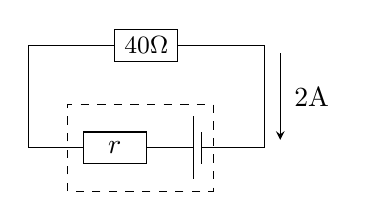
\begin{tikzpicture}[>=stealth]
        \draw(0.6,0.4)--(0.6,-0.4);
        \draw(0.7,0.2)--(0.7,-0.2);
        \draw(0.6,0)--(-1.5,0)--(-1.5,1.3)--(1.5,1.3)--(1.5,0)--(0.7,0);
        \draw[fill=white](-0.8,-0.2) rectangle (0,0.2);
        \node at(-0.4,0) {$r$};
        \draw[dashed] (-1,-0.55) rectangle (0.85,0.55);
        \draw[fill=white] (-0.4,1.1) rectangle (0.4,1.5);
        \node at(0,1.3) {\small $40\Omega$};
        \draw[->](1.7,1.2)--(1.7,0.1);
        \node at(2.1,0.65) {2A};
      \end{tikzpicture}
    \end{center}
  \end{minipage}
  \begin{minipage}{7cm}
    \begin{center}
      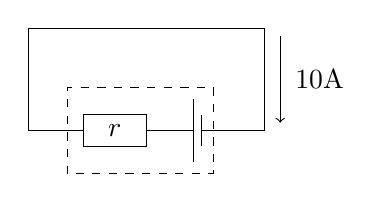
\begin{tikzpicture}
        \draw(0.6,0.4)--(0.6,-0.4);
        \draw(0.7,0.2)--(0.7,-0.2);
        \draw(0.6,0)--(-1.5,0)--(-1.5,1.3)--(1.5,1.3)--(1.5,0)--(0.7,0);
        \draw[fill=white](-0.8,-0.2) rectangle (0,0.2);
        \node at(-0.4,0) {$r$};
        \draw[dashed] (-1,-0.55) rectangle (0.85,0.55);
        \draw[->](1.7,1.2)--(1.7,0.1);
        \node at(2.2,0.65) {10A};
      \end{tikzpicture}
    \end{center}
  \end{minipage}
  \vspace{0.6cm}
  
  \begin{enumerate}[(${1}-$a)]
    \setlength{\itemsep}{15pt}
  \item 開放電圧を$v$とし, その抵抗を$r$ とする. 40$\Omega$の抵抗を加えたときの回路方程式は
    \begin{eqnarray*}
      2\cdot (40+r) = v 
    \end{eqnarray*}
    また, 端子を短絡したときの回路方程式は
    \begin{eqnarray*}
      10\cdot r = v
    \end{eqnarray*}
    これを解くと$v=100,\,r=10$, したがって, 開放電圧は\underline{\bf 100V}である.
  \item 端子を短絡すると10A流れて, 開放電圧は100Vであるから最大電力は
    \begin{eqnarray*}
      10\cdot 100 = \underline{\bf 1{\rm kW}}
    \end{eqnarray*}
  \item 回路図は以下のようにかける. ここで豆電球をILと表記する.
        \begin{center}
      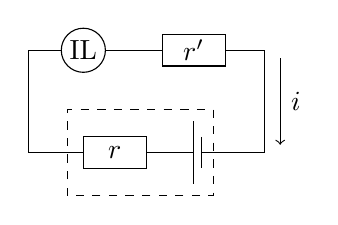
\begin{tikzpicture}
        \draw(0.6,0.4)--(0.6,-0.4);
        \draw(0.7,0.2)--(0.7,-0.2);
        \draw(0.6,0)--(-1.5,0)--(-1.5,1.3)--(1.5,1.3)--(1.5,0)--(0.7,0);
        \draw[fill=white](-0.8,-0.2) rectangle (0,0.2);
        \node at(-0.4,0) {$r$};
        \draw[dashed] (-1,-0.55) rectangle (0.85,0.55);
        \draw[->](1.7,1.2)--(1.7,0.1);
        \node at(1.9,0.65) {$i$};
        \draw[fill=white] (0.2,1.1) rectangle (1,1.5);
        \node at(0.6,1.3) {$r'$};
        \draw[fill=white] (-0.8,1.3) circle[radius=0.28];
        \node at(-0.8,1.3) {IL};
      \end{tikzpicture}
    \end{center}
    電球は50V, 100Wなので流れる電流は
    \begin{eqnarray*}
      i = 100\div 50 = 2{\rm A}
    \end{eqnarray*}
    となる. ゆえに回路の方程式は
    \begin{eqnarray*}
      &&ir+ir' = v-50\\
      \Longleftrightarrow\ && 2\cdot 10+2r' = 50\\
      \Longleftrightarrow\ && r' = 15
    \end{eqnarray*}
    よって, 抵抗の値を\underline{\bf 15$\Omega$}にすればよい.
  \end{enumerate}
\end{enumerate}
\newpage
\section{}
\subsection{情報通信ネットワーク}
\subsubsection{問題文}
\begin{enumerate}[(1)]
  \setlength{\itemsep}{15pt}
\item OSI参照モデル(OSI\ reference model) のプロトコル階層(protocol hierarchy)のうち, 以下に該当する階層の名称を答えよ。
  \begin{enumerate}[(${1}-$a)]
    \setlength{\itemsep}{5pt}
  \item 主として物理的に隣接する機器間の通信を行う機能を実現する階層
  \item  ネットワークの末端に接続された機器間の通信を行う機能を実現する階層
  \end{enumerate}
\item TCPでは服装ウィンドウ(congestion window)を使ったフロー制御(flow control)が行われる。\\
  TCP Renoにはスロースタートフェーズ(slow start phase)と輻輳回避フェーズ(congestion avoidance phase)という二つの状態が定義されている。ネットワークが混雑していないと仮定したときに, 輻輳ウィンドウサイズがどのように増加するのか, スロースタートフェーズと輻輳回避フェーズの場合についてそれぞれ説明せよ。
\item あるコンピュータのIPアドレスとサブネットマスクが192.168.100.226/28であるとする。このコンピュータが属するサブネットのネットワークアドレスとブロードキャストアドレスを答えよ。
\item 以下の図はある Autonomous Systemの構成を表すものとする。辺(edge)に付与された数字は各辺のコストとする。Router1,\ 2,\ 3,\ 4を結ぶ辺はブロードキャスト接続(broadcast link)を表し, そのコストは1である。このとき, NW AからNW Dまでの経路として, RIPとOSPFそれぞれによって選択される経路を答えよ。\\
  \begin{center}
    \includegraphics[width=10cm]{net.png}
  \end{center}
\item CSMA/CDとCSMA/CAの違いを説明せよ。
\end{enumerate}
\newpage

\subsubsection{解答例}
\begin{enumerate}[(1)]
  \setlength{\itemsep}{15pt}
\item OSI参照モデルについて以下に示す.
  \begin{center}
    \begin{tabular}{|c|c|} \hline
      第7層&アプリケーション層 \\ \hline
      第6層&プレゼンテーション層 \\ \hline
      第5層&セション層 \\ \hline
      第4層&トランスポート層 \\ \hline
      第3層&ネットワーク層 \\ \hline
      第2層&データリンク層 \\ \hline
      第1層&物理層 \\ \hline
    \end{tabular}
  \end{center}
  \begin{itemize}
  \item 物理層 … 機器と機器とを「物理的につなぐ」ことに関してルールを定める層
  \item データリンク層 … 「同じネットワーク内」にいる通信機器とのやり取りに関してルールを定める層
  \item ネットワーク層 … 「異なるネットワーク」とのやり取りに関してルールを定める層
  \item トランスポート層 … 「データの品質管理」に関してルールを定める層
  \item セション層 … 「最終的な通信の目的にあわせた送受信管理」のルールを定める層
  \item プレゼンテーション層 … 「データの表現形式」について取り決める層
  \item アプリケーション層 … 「アプリケーションソフトがやり取りする情報」について取り決める層
  \end{itemize}
  \vspace{0.3cm}
  
  \begin{enumerate}[({1}$-$a)]
    \setlength{\itemsep}{5pt}
  \item 物理的に隣接する機器間の通信なので\underline{\bf 物理層}
  \item ネットワークの末端, つまり同じnネットワーク内の通信なので, \underline{\bf データリンク層}
  \end{enumerate}
\item 
\end{enumerate}
\index{ティック@tikz}
% \printindex

\end{document}
